\documentclass{article}
\usepackage{qilin}
\title{MSE160 \\ Problem Set \# 1}
\author{QiLin Xue}
\lhead{MSE160}
\rhead{QiLin Xue}

\begin{document}
    \maketitle
    \section*{Problem One}
    The force between two atoms can be modelled using the Lennard Jones potential, which gives rise to the force diagram shown below, represented in purple.
    \begin{center}
        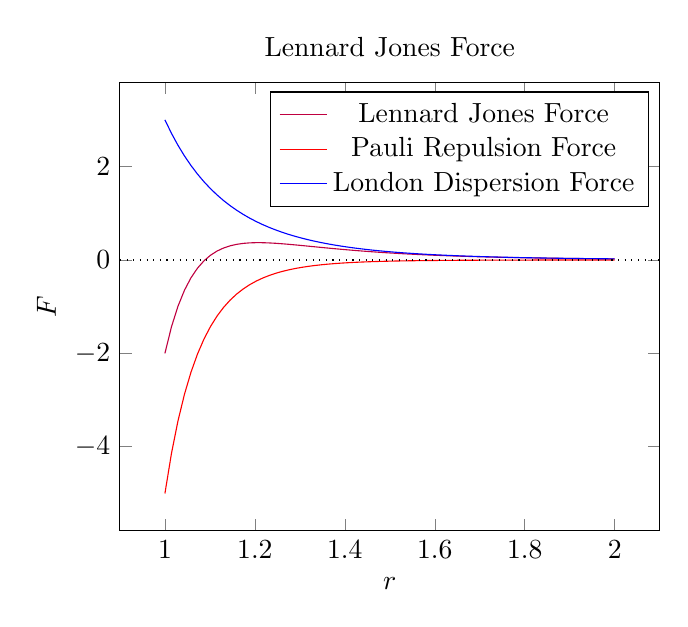
\begin{tikzpicture}
        \begin{axis}[
        % legend pos=outer north east,
        title=Lennard Jones Force,
        axis lines = box,
        xlabel = $r$,
        ylabel = $F$,
        variable = t,
        trig format plots = rad,
        ]
        \addplot [
            domain=1:2,
            samples=70,
            color=purple,
            ]
            {-5/x^13+3/x^7};
            \addlegendentry{Lennard Jones Force}
            \addplot [
                domain=1:2,
                samples=70,
                color=red,
                ]
            {-5/x^13};\addlegendentry{Pauli Repulsion Force}
            \addplot [
                domain=1:2,
                samples=70,
                color=blue,
                ]
            {+3/x^7};\addlegendentry{London Dispersion Force}
        \draw[dotted] (0.9, 0) -- (2.1, 0);
        \end{axis}
        \end{tikzpicture}
    \end{center}
    \textbf{(a)} There are two competing interactions. The physical proximity of the electrons results at short distances results in a large pauli repulsion force. At larger distances, the two neutral atoms become an induced dipole via a phenmenon known as london dispersion. This causes an attraction force to dominate at far distances. As a result, from the intermediate value theorem, there has to be a location of zero force in between the two extremes. This is represented by the intersection point of the force with the horizontal axis.
    \vspace{2mm}

    \noindent \textbf{(b)} If we assume the atoms displace very small distances from their equilibrium location, then we can write the restoring force between the two atoms as:
    \begin{equation}
        F = -k\Delta x
    \end{equation}
    where:
    \begin{equation}
        k = \frac{EA}{L}.
    \end{equation}
    where $A$ is the relevant sectional area of the atom, $L$ as the bond length, and $E$ is defined as the Young's Modulus. This means that the Young's Modulus is proportional to the slope at equilibrium:
    \begin{equation}
        E \propto \frac{dF}{dr}\Biggr|_{r=r_0}
    \end{equation}
    which is in turn determined by quantum dynamical properties of the atom which tells us how polarizable the electrons are and how strong the Pauli repulsion is. The only way to change the Young's Modulus is to change these two properties, which is fundamental to a material. Changing these would imply the actual type of material changed as well.
    \section*{Problem Two}
    Let the strain in the diameter be $\varepsilon_d$. The maximum strain we can accept is:
    \begin{equation}
        \varepsilon_{d,\text{max}} = \frac{9.5 \times 10^{-3}\si{\milli\meter}}{12.5\si{\milli\meter}} = 7.6\times 10^{-4}
    \end{equation}
    The applied stress is:
    \begin{equation}
        \sigma = \frac{F}{\pi d^2/4} = \frac{30 \times 10^3 \si{\newton}}{\frac{\pi}{4}\times (12.5 \si{\milli\meter})^2} = 244\si{\mega\pascal}
    \end{equation}
    The longitudinal strain is:
    \begin{equation}
        \varepsilon_{\ell} = \frac{\sigma}{E}
    \end{equation}
    and using the Poisson's ratio $\nu = 0.3$, we can calculate the strain in the diameter to be:
    \begin{equation}
        \varepsilon_d = \nu \frac{\sigma}{E}
    \end{equation}
    Using the maximum strain we calculated from earlier, we can calculate the minimum Young's Modulus to be:
    \begin{equation}
        E_\text{min} = \frac{\nu \sigma}{\varepsilon_{d,\text{max}}} = \frac{0.3 \cdot 244 \times 10^6 \si{\pascal}}{7.6 \times 10^{-4}} = 96.3 \si{\giga\pascal}
    \end{equation}
    To select possible materials, it needs to satisfy two constraints. The yield strength must first be greater than $\sigma$ and the Young's Modulus must be larger than $E_\text{min}$. The only two that satisfy this is $\boxed{\text{brass and steel}}$.
    \section*{Problem Three}
    Let us first answer what the maximum length the sample could elongate to under purely elastic deformation. This occurs for stress values of up to the yield strength of $600\si{\mega\pascal}$. We have:
    \begin{equation}
        \varepsilon_\text{max} = \frac{\Delta L_\text{max}}{L} = \frac{\sigma}{E} \implies \Delta L_\text{max} = \frac{L\sigma}{E} = \frac{(500\si{\milli\meter})(600\times 10^6 \si{\pascal})}{200 \times 10^9 \si{\pascal}} = \boxed{1.5\si{\milli\meter}}
    \end{equation}
    As a result, the bar is undergoing $\boxed{\text{plastic deformation}}$ as the actual elongation of $6\si{\milli\meter}$ is longer than the maximum elastic elongation.
    \section*{Problem Four}
    \textbf{(a)}
    We first check that the cylinder undergoes elastic deformation by calculating the stress:
    \begin{equation}
        \sigma = \frac{F}{\frac{\pi}{4} d^2} = \frac{1700\si{\newton}}{\frac{\pi}{4}(10\si{\milli\meter})^2} = 21.6\si{\mega\pascal}
    \end{equation}
    which is below the yield strength. The elongation would then be:
    \begin{equation}
        \varepsilon = \frac{\Delta L}{L} = \frac{\sigma}{E} \implies \Delta L = \frac{L \sigma}{E} = \frac{(300\si{\milli\meter})(21.6\times 10^6 \si{\pascal})}{68\times 10^9 \si{\pascal}} = \boxed{0.0953 \si{\milli\meter}}
    \end{equation}
    \textbf{(b)} The Poisson's ratio can be calculated given the Young's Modulus and the Shear Modulus:
    \begin{equation}
        E = 2G(1+\nu) \implies \nu = \frac{E}{2G}-1 = 0.3077
    \end{equation}
    The longitudinal strain is:
    \begin{equation}
        \varepsilon_\ell = \frac{\sigma}{E} = \frac{21.6\times 10^6 \si{\pascal}}{68\times 10^9 \si{\pascal}} = 3.176 \times 10^{-4}
    \end{equation}
    and we can relate this to the strain in the diameter via:
    \begin{equation}
        \varepsilon_d = \frac{\Delta d}{d} = \nu \epsilon_\ell \implies \Delta d = d\nu\varepsilon_\ell = (10\si{\milli\meter})(0.3077)(3.176\times 10^{-4})
    \end{equation}
    and the final diameter is:
    \begin{equation}
        d_f = d - \Delta d = 9.999 \si{\milli\meter}
    \end{equation}
    \section*{Problem Five}
    \textbf{(a)}
    The stress needed for the plate to break in the lower half is given by:
    \begin{equation}
        \sigma = \frac{3FL}{2wh^2} \implies F \propto \frac{wh^2}{L}
    \end{equation}
    In the second test, the height changes by a factor of $\frac{5}{7}$, the width changes by a factor of $\frac{7.5}{10}$. Since the length is constant, the force changes by a factor of:
    \begin{equation}
        \frac{F_\text{new}}{F_\text{old}} = \frac{7.5}{10} \left(\frac{5}{7}\right)^2 = 0.3827
    \end{equation}
    so the new plate will break at a force of $F = 0.3827 \cdot 5000 \si{\newton} = \boxed{1913\si{\newton}}$.
    \vspace{2mm}

    \textbf{(b)} Well I'm not really sure what I'm expected to write here, since we already discussed three major reasons in class. However, ceramics being very brittle is a huge contributing factor to everything. It will be difficult to be shaped into a dogbone shape without it breaking. To overcome the restoring force, the machine also needs to grip it super tightly and that can often cause the material to crumble. Below, I have copied the strain vs stress curve of ceramics, metals, and polymers:
    \begin{figure}[ht]
        \centering
        \incfig{stress_strain}
    \end{figure}
    As we can see, ceramics also have a high Young's Modulus. This means that strains are often very small and hard to detect, and it can quickly reach failure.
\end{document}

